\documentclass[a4paper]{report}
\usepackage{amsmath}
\usepackage{bm}
\usepackage{amsfonts}
\usepackage{MnSymbol}
\usepackage{graphicx}

\title{Gruppövning 1 - Grupp A19}
\author{Max Hagman, Felix Bjerhem Aronsson}
\begin{document}

\maketitle

\chapter{Teoriövningar}
\begin{enumerate}
    % 1
    \item 
        \begin{enumerate}
            % a
            \item 
                Formeln för en triangels area är $\frac{b \cdot h}{2}$.
                Utgår man ifrån detta så får man att basen kan representeras av $||\overrightarrow{P_{1}P_{3}}||$ (eller $\overrightarrow{P_{1}P_{2}}$).
                Höjden, däremot, går inte att representera direkt utav någon vektorn baserad på punkterna $P_{1}$, $P_{2}$ och $P_{3}$.
                För att få höjden tar man $\overrightarrow{P_{1}P_{2}}$ projektion på den linje som har riktningsvektor $\overrightarrow{P_{1}P_{3}}$, 
                som blir basen till en triangel med $||\overrightarrow{P_{1}P_{2}}||$ som hypotenusa.
                Enligt Pytagoras sats kan man då få höjden på denna nya triangel genom $\sqrt{ ||\overrightarrow{P_{1}P_{2}}||^{2} - (\frac{|\overrightarrow{P_{1}P_{3}}\cdot \overrightarrow{P_{1}P_{2}}|}{||\overrightarrow{P_{1}P_{3}}||})^{2}}$.
                Om man sedan multiplicerar denna höjden, med $||\overrightarrow{P_{1}P_{3}}||$ så får man formeln för triangelns area enligt följande:\\
                \begin{equation}
                        \frac{\sqrt{ ||\overrightarrow{P_{1}P_{2}}||^{2} - (\frac{|\overrightarrow{P_{1}P_{3}}\cdot \overrightarrow{P_{1}P_{2}}|}{||\overrightarrow{P_{1}P_{3}}||})^{2}}\cdot ||\overrightarrow{P_{1}P_{3}}||}{2}
                \end{equation}

                \begin{center}
                    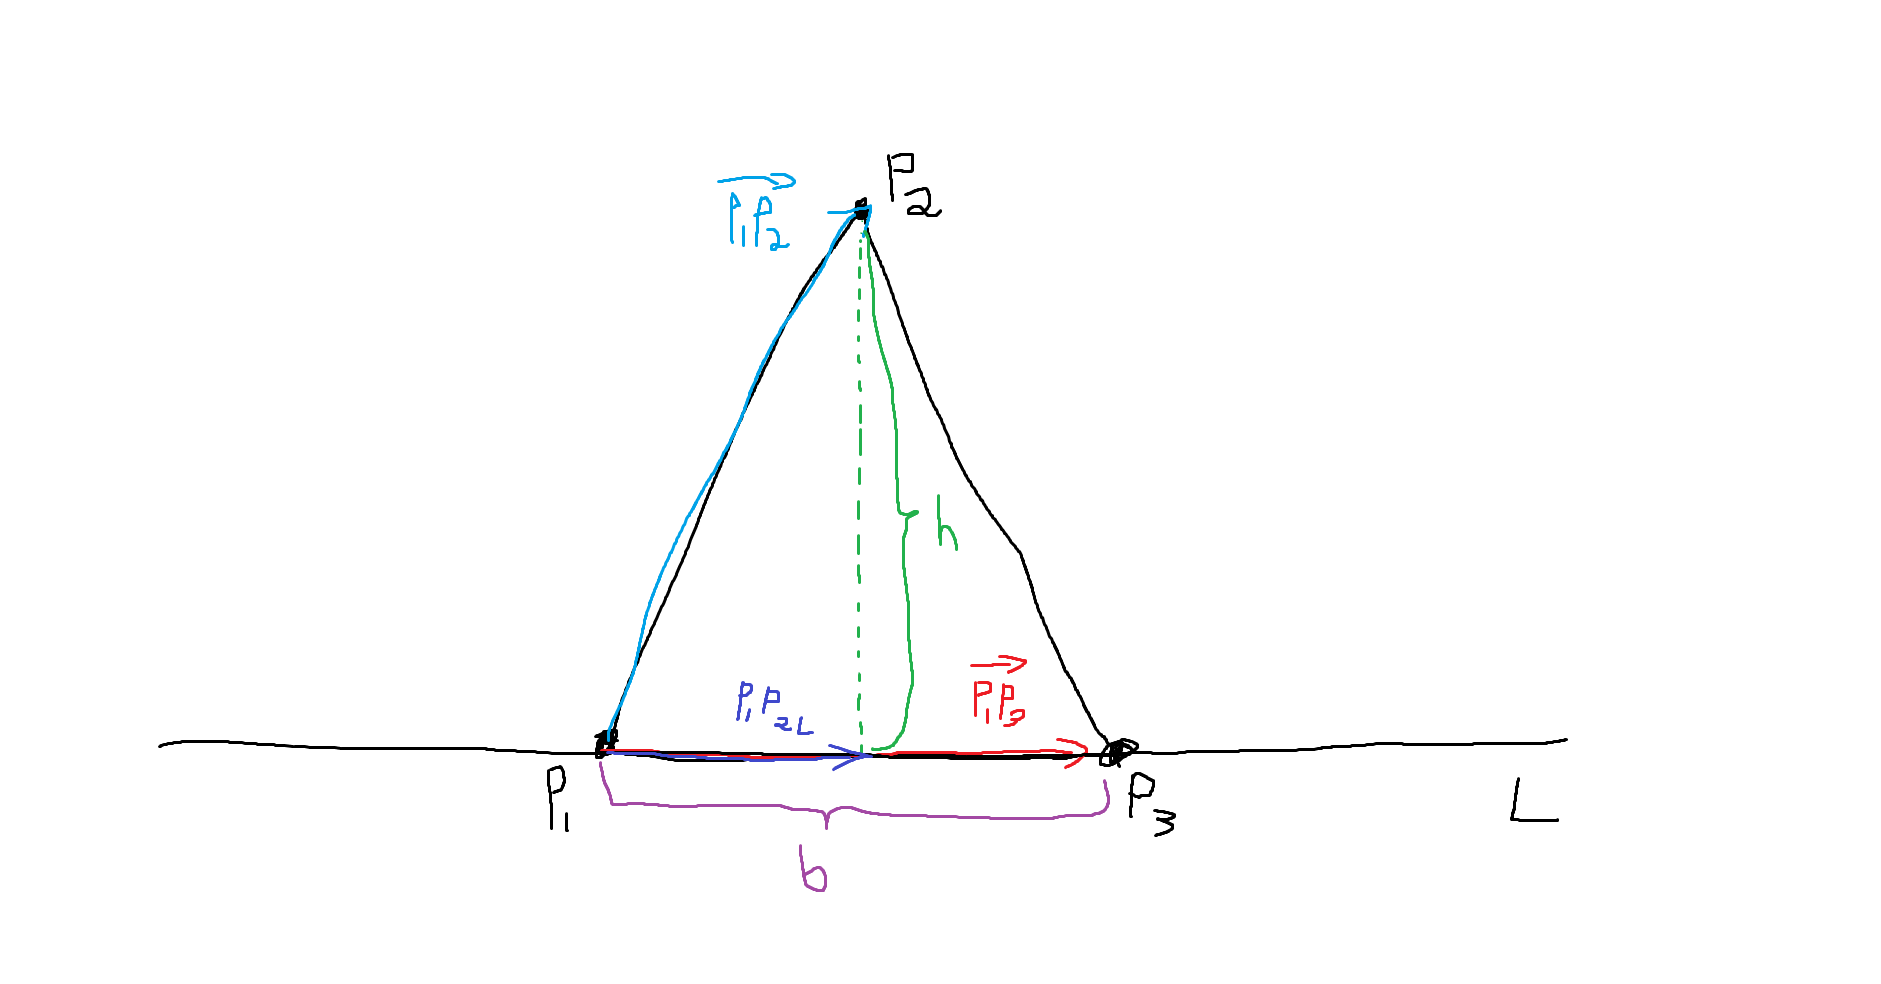
\includegraphics[scale=0.15]{bild.png}
                \end{center}

                Om vi sedan applicerar denna formel på triangeln med hörnen $P_{1}=(1,1)$, $P_{2}=(4,2)$ och $P_{3}=(-1,7)$, så har vi vektorerna:\\
                \begin{center}
                    $\bm{v} = P_{1}-P_{2} = \begin{pmatrix}5\\-5\end{pmatrix}$\\
                    $\bm{u}=P_{1}-P_{3} = \begin{pmatrix}2\\-6\end{pmatrix}$\\
                \end{center}
                
                Om man sedan kan stoppa in i formeln för att få arean:
                \begin{equation}
                    \frac{\sqrt{||\bm{v}||^{2}-(\frac{|\bm{u}\cdot \bm{v}|}{||\bm{u}||})^{2}}\cdot ||\bm{u}||}{2}=
                    \frac{\sqrt{\sqrt{50}^{2}-(\frac{5\cdot 2 + (-5)\cdot (-6)}{\sqrt{40}})^{2}}\cdot \sqrt{40}}{2}=
                    10
                \end{equation}
            % b
            \item 
                Med tre godtyckliga punkter på en linje, $P_{a}$, $P_{b}$ och $P_{c}$, kan vi bilda tre st vektorer, $\bm{v}$, $\bm{u}$ och $\bm{w}$.
                Då punkterna ligger på en linje får alla vektorer samma riktning.
                Alltså är minsta vinkeln, $\alpha$, blir då 0.
                Uttrycket i roten ur blir då: 
                \begin{center}
                    $
                    ||\bm{v}||^{2}-(\frac{|\bm{u}\cdot \bm{v}|}{||\bm{u}||})^{2} = 
                    ||\bm{v}||^{2}-(\frac{||\bm{u}||\cdot||\bm{v}||cos(0)}{||\bm{u}||})^{2}=
                    ||\bm{v}||^{2}-||\bm{v}||^{2}=0
                    $
                \end{center}
                Detta leder till att vi får: $\frac{\sqrt{0}\cdot ||\bm{u}||}{2}=\frac{0}{2}=0$.
                Alltså är arean av den triangeln som $P_{a}$, $P_{b}$ och $P_{c}$ bildar 0.
        \end{enumerate}
    \item
        I en rätvinklig triangel $ABC$ med vinkeln vid $B=\frac{\pi}{2}$.\\
        Vi definierar triangelns vektorer som $\bm{u} = \overrightarrow{AB}$, $\bm{v} = \overrightarrow{BC}$ och $\bm{u}+\bm{v} = \overrightarrow{AC}$.
        \begin{center}
            $||\bm{u}||^{2}+||\bm{v}||^{2}=||\bm{u}+\bm{v}||^{2}=(\bm{u}+\bm{v})\cdot (\bm{u}+\bm{v}) = \bm{u}\cdot \bm{u} + 2\bm{u}\cdot \bm{v}+\bm{v}\cdot \bm{v}$\\
        \end{center}
        Då $\bm{u}\cdot \bm{u}=||\bm{u}||^{2}$ och $\bm{v}\cdot \bm{v}=||\bm{v}||^{2}$ får vi $||\bm{u}+\bm{v}||^{2}=||\bm{u}||^{2}+||\bm{v}||^{2}+2\bm{u}\cdot \bm{v}$.\\
        Då $\bm{u}$ och $\bm{v}$ är ortogonala blir $2\bm{u}\cdot \bm{v} = 0$ vilket ger oss: $||\bm{u}||^{2}+||\bm{v}||^{2} \blacksquare$
    \item 
        \begin{enumerate}
            \item 
                Då $\bm{b}\times \bm{c}$ ger normalen, vilket är ortogonal till planet $\bm{bc}$ spänner. 
                Detta leder till att vi får $\bm{a}\times \bm{n}$ som sedan är ortogonal mot normalen, dvs parallell med planet.
                Eftersom den är parallell med planet, innebär det att normalens normal vektor kan representeras av någon linjär kombination av $\bm{b}$ och $\bm{c}$,
                dvs $\lambda\bm{b} + \mu\bm{c}$.
                \begin{center}
                    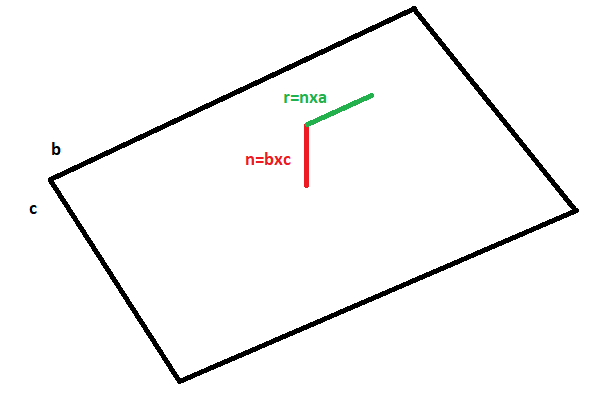
\includegraphics[scale=0.4]{bild2.png}
                \end{center}
            \item
                Då $\bm{a}\times (\bm{b}\times \bm{c})$ är parallell med planet är det också ortogonalt mot $\bm{a}$.
                Skalärprodukten av två vektorer som är ortogonala mot varandra är 0.
                Sedan kan vi skriva om $\lambda(\bm{a}\cdot\bm{b}) + \mu(\bm{a}\cdot\bm{c})$ som:
                \begin{center}
                    $\lambda(\bm{a}\cdot\bm{b}) + \mu(\bm{a}\cdot\bm{c})=$
                    $\lambda(\bm{b}\cdot\bm{a}) + \mu(\bm{b}\cdot\bm{a})=$\\
                    $\lambda\bm{b}\cdot\bm{a} + \mu\bm{b}\cdot\bm{a}=$
                    $\bm{a}\cdot(\lambda\bm{b} + \mu\bm{c})$
                \end{center}
                Och eftersom $\lambda\bm{b} + \mu\bm{c} = \bm{a}\times (\bm{b}\times \bm{c})$,
                innebär det att $\lambda\bm{b} + \mu\bm{c}$ är ortogonalt mot $\bm{a}$ och då blir $\lambda(\bm{a}\cdot\bm{b}) + \mu(\bm{a}\cdot\bm{c}) = 0$.

            \item
                Då $\lambda (\bm{a}\cdot \bm{b})+\mu (\bm{a}\cdot \bm{c})=0 \Leftrightarrow \begin{pmatrix}\lambda\\\mu\end{pmatrix} \cdot \begin{pmatrix}\bm{a}\cdot \bm{b}\\ \bm{a} \cdot \bm{c} \end{pmatrix} = 0$\\
                kan vi räkna ut att 
                \begin{center}
                    $\begin{pmatrix}\bm{a}\cdot \bm{c}\\ \bm{-a} \cdot \bm{b} \end{pmatrix}\cdot\begin{pmatrix}\bm{a}\cdot \bm{b}\\ \bm{a} \cdot \bm{c} \end{pmatrix} = (\bm{a}\cdot\bm{c})(\bm{a}\cdot\bm{b})-(\bm{a}\cdot\bm{b})(\bm{a}\cdot\bm{c})=0$.
                \end{center}
                Detta innebär att $\begin{pmatrix}\lambda\\\mu\end{pmatrix}$ och $\begin{pmatrix}\bm{a}\cdot \bm{c}\\ \bm{-a} \cdot \bm{b} \end{pmatrix}$ är ortogonala mot $\begin{pmatrix}\bm{a}\cdot \bm{b}\\ \bm{a} \cdot \bm{c} \end{pmatrix}$ och
                därför måste de vara parallella.\\\\
                Vilket implicerar att man kan skriva den ena vektorn som en linjärkombination av den andra vektorn, såsom:
                \begin{center}
                    $\begin{pmatrix}\lambda\\\mu\end{pmatrix}=s\begin{pmatrix}\bm{a}\cdot\bm{c}\\ (-)\bm{a}\cdot\bm{b}\end{pmatrix}$, $s \in \mathbb{R}$
                \end{center}
            \item
                Då vi antar att $s=1$ ser ekvationen ut som följande:
                \begin{center}
                    $\begin{pmatrix}\lambda\\\mu\end{pmatrix}=\begin{pmatrix}\bm{a}\cdot c\\ (-\bm{a})\cdot \bm{b}\end{pmatrix}$
                \end{center}
                Om vi då sätter
                $a=\begin{pmatrix}3\\1\\5\end{pmatrix}$, $b=\begin{pmatrix}1\\4\\2\end{pmatrix}$ och $c=\begin{pmatrix}2\\3\\1\end{pmatrix}$\\
                \begin{center}
                    $\bm{a}\cdot \bm{c} = 3\cdot 2 + 1\cdot 3 + 5\cdot 1 = 6 + 3 + 5 = 14 = \lambda$\\
                    $-\bm{a}\cdot \bm{b} = -3\cdot 1 - 1\cdot 4 - 5\cdot 2 = -3 -4 -10 = -17 = \mu$
                \end{center}
                Med hjälp av dessa värden kan vi sätta:
                \begin{center}
                    $\lambda \bm{b} + \mu \bm{c} = 
                    14\begin{pmatrix}1\\4\\2\end{pmatrix} + (-17)\begin{pmatrix}2\\3\\1\end{pmatrix} =
                    \begin{pmatrix}-20\\5\\11\end{pmatrix}$
                \end{center}
                Om vi dessutom räknar ut $\bm{a}\times(\bm{b}\times\bm{c})$ får vi $\begin{pmatrix}-20\\5\\11\end{pmatrix}$.
        \end{enumerate}
\end{enumerate}

\chapter{Datorövningar}
\begin{enumerate}
    % 1
    \item Se Span.m för implementation
    % 2
    \item \begin{enumerate}
        % a
        \item 
            Se NormalNormalisedVektor.m för implementation.\\
            Vi börjar med att räkna ut den normalen till planet som spänns av u,v.
            Detta görs med matlab funktionen cross() som räknar ut kryssprodukten.
            För att normalisera normalen delas den på sin längd, vilket man får från norm(x,1).
            Sedan returneras normalen.
        % b
        \item 
            Se OrtoProj.m för implementation.\\
            Funktionen använder sig utav formeln:
            \begin{displaymath}
                \bm{v}-\frac{\bm{v}\times \bm{n}}{||\bm{n}||^{2}}\cdot \bm{n}
            \end{displaymath}
            Med denna beräknar den projektionen av given vector på planet utifrån normalen.
        % c
        \item 
            Se test.m för att testa alla funktioner tillsammans.\\
            Vi använder oss utav NormalNormalisedVektor.m för att få en normal som vi sedan skickar in till OrtoProj.m med våran punkt.
            Detta ger oss resultatet $\begin{pmatrix}0\\e\\1\end{pmatrix}$. 
            Vilket är projektionen av $P = \begin{pmatrix}\pi\\e\\1\end{pmatrix}$ på \emph{xy}-planet.
    \end{enumerate}
    \item Se TriangelToPlain.m för implementation.
\end{enumerate}
\end{document}